%%
%% Copyright 2007, 2008, 2009 Elsevier Ltd
%%
%% This file is part of the 'Elsarticle Bundle'.
%% ---------------------------------------------
%%
%% It may be distributed under the conditions of the LaTeX Project Public
%% License, either version 1.2 of this license or (at your option) any
%% later version.  The latest version of this license is in
%%    http://www.latex-project.org/lppl.txt
%% and version 1.2 or later is part of all distributions of LaTeX
%% version 1999/12/01 or later.
%%
%% The list of all files belonging to the 'Elsarticle Bundle' is
%% given in the file `manifest.txt'.
%%

%% Template article for Elsevier's document class `elsarticle'
%% with numbered style bibliographic references
%% SP 2008/03/01
%%
%%
%%
%% $Id: elsarticle-template-num.tex 4 2009-10-24 08:22:58Z rishi $
%%
%%
\documentclass[preprint,12pt,3p]{elsarticle}

%% Use the option review to obtain double line spacing
%% \documentclass[preprint,review,12pt]{elsarticle}
\usepackage{graphicx}
\usepackage{amssymb}
%% The amsthm package provides extended theorem environments
%% \usepackage{amsthm}

%% The lineno packages adds line numbers. Start line numbering with
%% \begin{linenumbers}, end it with \end{linenumbers}. Or switch it on
%% for the whole article with \linenumbers after \end{frontmatter}.
%% \usepackage{lineno}

\usepackage{float}
\usepackage{subcaption}
\usepackage{listings}

% Possible journals:
% - Journal of Marketing Research Q1
% - Journal of Interactive Marketing Q1
\journal{Journal of Interactive Marketing}

\begin{document}

\begin{frontmatter}

% TODO: Think in a better title
\title{Visualizing website traffic}

\author[label1]{Fernando G\'{o}mez-Herrera}
\address[label1]{Instituto Tecnol\'{o}gico y de Estudios Superiores de Monterrey (ITESM)}
\ead{gomezhyuuga@acm.org}
%\ead[url]{github.com/gomezhyuuga}
\author[label1]{Ra\'{u}l Monroy Borja}
\ead{raulm@itesm.mx}

\author[label2]{Dante Dessavre}
\ead{dgamades@stevens.edu}
\author[label2]{Jos\'{e} Ram\'{i}rez M\'{a}rquez}
\ead{jmarquez@stevens.edu}
\address[label2]{Stevens Institute of Technology (Stevens)}



\begin{abstract}
Digital advertising has become one of the most popular business model for many companies REF. Thus, the need of tools for analyzing and measuring digital content has become an important area of interest in past few decades. Nowadays there are common standards for measuring digital content, from web site traffic (page views, bounce rate, session count) to advertising campaigns effectiveness (conversion rate, funnel techniques). Most commonly the use of text reports are used for presenting such analytics. The present work provides a tool for analyzing graphically the interactions of users in web sites, proposing new layouts for displaying visits and enabling powerful detections like browsing patterns, profiling objective pages or even spot visitor clusters.
\end{abstract}

\begin{keyword}
%% keywords here, in the form: keyword \sep keyword
web analytics traffic-analysis
%% MSC codes here, in the form: \MSC code \sep code
%% or \MSC[2008] code \sep code (2000 is the default)
\end{keyword}

\end{frontmatter}

%%
%% Start line numbering here if you want
%%
% \linenumbers

%% main text
\section{Introduction}
\label{sec:intro}
Web analytics has become an important area of research in the past few years REF. With companies building their business models based on advertising, it is very important to have tools for measuring digital content interactions such as number of page views, session count, demographics and other commonly defined metrics like \textit{bounce rate, exit rate, conversions, etc.}, using such tools you can get to know better your audience and so what are their preferences, what is the content they like, how much time spend reading or view content and also the browsing behavior inside your website.
Big companies like Google are aware of such need of tools in the market and because that advertising is their main business model, they have been creating tools for their customers to analyze digital metrics. The most popular services provided by Google are Google Analytics and DoubleClick. Both tools can be used to measure web advertising campaigns and they provide predefined reports for that. Of course Google is not the only one in the advertising market, Yahoo, Microsoft, Amazon and even Facebook have their own tools and services for their platforms.


\section{Previous work}
\label{sec:background}
There are many tools available for measuring digital content and because this is such an important topic in the \textit{marketing} industry, some companies have created their own tracking tools and build a business around it. We will analyze such tools dividing them into two categories: \textit{enterprise solutions} and \textit{open source} tools. Many of the enterprise solutions (with the exception of Google products) are paid services whereas the open source tools are free to use.

% TODO: link to each service website

\subsection{Enterprise solutions}
\textbf{Google Services}.
As the biggest company in the Internet, Google has three main products focused on web advertising (Google AdWords and DoubleClick) and web analytics (Google Analytics). Combining such products you can have powerful insights of the users that are visiting your website. DoubleClick is a paid service, but AdWords and Analytics are free to use.

Google Analytics is the main product for getting reports and analyze the traffic to a website. It can be configured to import and track ad campaigns from AdWords and DoubleClick, and allows you to segment the traffic from many sources and with many filters as you want. Also it has the advantage for being widely known by marketing experts and people in many areas so it has become a standard in a certain way.

\textbf{comScore}.
It is an American company founded in Virginia which now has big presence not only in the Internet but also providing services to other kind of media companies like the TV industry, newspapers, health care and others as well. Nevertheless, we can not get a further analysis of their tools because they are paid services and usually oriented to big companies with large amount of data. Despite of this fact, comScore has been very open with their current research and publishing some reports in a periodic way \cite{comScoreIVT, BrianPugh2012}.

\textbf{KissMetrics}.
Also a paid service but this company focuses in more tailored need experience, focusing on consulting and teaching their customers how to implement the tool and interpret the results. Popular stories about the use of KissMetrics are the one of LucidChart (https://www.kissmetrics.com/lucidchart/), a tool for creating digital diagrams, which after upgrading their product, needed to measure the performance of the new design and by using KissMetrics, they could determine an increase of 30\% more conversions. Another case is the one of the e-commerce site Manillo, an Amazon-like service in Denmark, which increased their ROI by 50\% by understanding better their audience (https://www.kissmetrics.com/manillo/).


The previous tools can only be tested as a hosted service. This is a disadvantage for some companies that need to complain with law regulations about the storing the customer's data or for companies that need an on-premise solution. Another big concern about this kind of services is that usually you do not own the data, instead you only have access to it through a third-party.

\subsection{Open Source tools}                                                                                               
\textbf{Piwik}.
One of the most popular and robust tools that could be self-hosted or as a service in the cloud. Piwik is a company that focuses on giving their users a complete control of everything, meaning that you get full reports (no data sampling), you are the owner of the 100\% of your data and also it is completely open source, which means that you can customize it as you wish. It is developed in PHP and also provides an HTTP API for consulting the reports.

\textbf{Open Web Analytics (OWA).}
Although this project has not published any new version since 2014, it is still popular in legacy websites. It was integrated in former versions of Content Management Systems like Wordpress or Media Wiki. It can be tested only by installing it on a personal server. One of the greatest features included out of the box is the \textit{click heatmap} that shows the \textit{hottest} sections of your pages.

\subsection{Common concepts}
The following terms are commonly used for referring to the performance of a website or an advertising campaign. It must be mentioned that each service provide their own implementation for computing the values and it is very common for the tools to disagree with the results.

\begin{itemize}
  \item Page View. Number of times a page was viewed by an user. A user can view the same o many pages multiple times in each visit.
  \item Visit. A collection of events from a user in a given period of time. A visit can contain multiple page views, downloads, clicks or any custom event triggered. Usually platforms setup a \textit{idle time} to finish the visit, i.e. if the user did not make any action within a window of time (e.g. 30 mins), then his/her visit is \textit{closed.} After that, any action would be considered as a new visit. The terms \textit{visit} or \textit{session} are used interchangeably within platform services.
  \item Bounce Rate. This is commonly used as a Key Performance Indicator (KPI) of how your pages are performing. It indicates the number of users that only view one page and leave immediately. The measure is more meaningful when used for single pages or goals, instead of using it in a global way.
  \item Objective/Goal. Custom defined event that gives to your company value or even revenue. Common objectives are: page views of selected pages (cart, about us, offers); for e-commerce adding an item to the cart, making a purchase, the checkout page; for media sites playing a video, watching a video for at least X seconds, etc. Each company define their objectives according to their business and needs.
  \item Conversion. Amount of users that triggered or \textit{achieved} an objective. For example how many times an objective page was uniquely visited, how many purchases have been made, number of checkouts, times an advertisement was seen, etc. Each conversion normally has associated a revenue for the company so increasing the conversions is a KPI for any analyst.
\end{itemize}

A complete description of other terms used in media analytics can be found in a report made by the Web Analytics Association (waa) \cite{Waa2007}.

As an example of how the platforms present the previous metrics, Figure \ref{fig:screenshots} shows examples of some of their reports.

% TODO: check positioning
\begin{figure}[h]
	\centering
	\begin{tabular}{cc}
		\subcaptionbox{
		Google Analytics: home dashboard \vspace{2 mm}
		\label{fig:ga_home}}{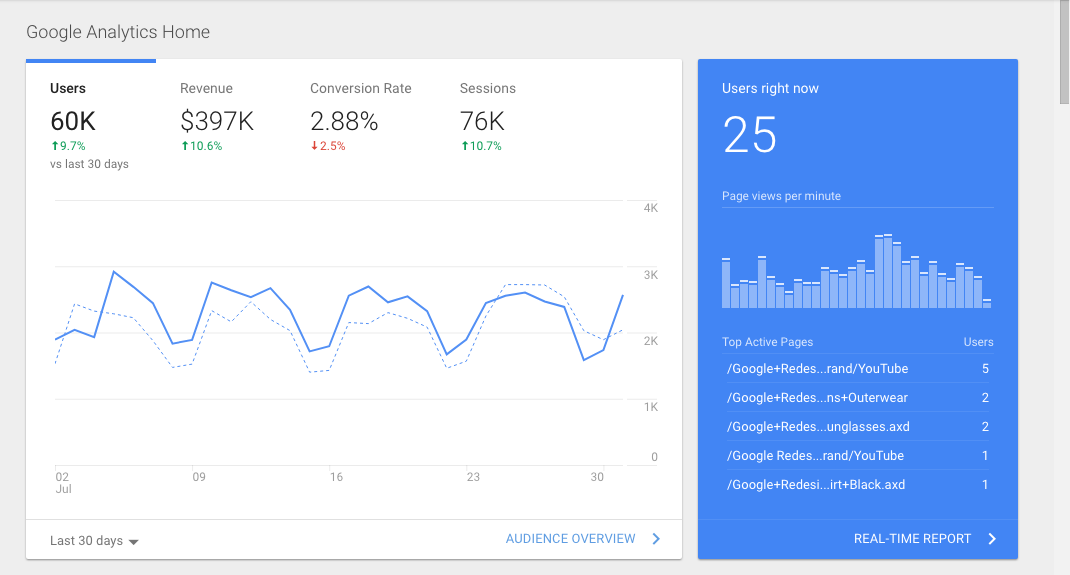
\includegraphics[width = 0.5\textwidth]{screenshots/analytics_home}} &
		\subcaptionbox{
		Google Analytics: funnel analysis \vspace{2 mm}
		\label{fig:ga_funnel}}{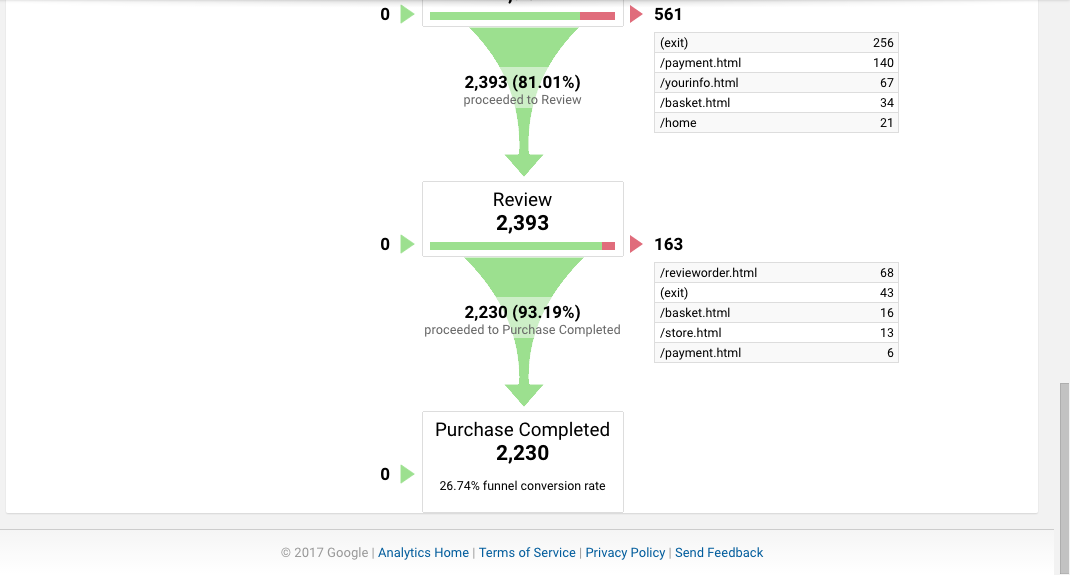
\includegraphics[width = 0.5\textwidth]{screenshots/analytics_funnel}} \\
		\subcaptionbox{
		Piwik: home dashboard \vspace{2 mm}
		\label{fig:piwik_home}}{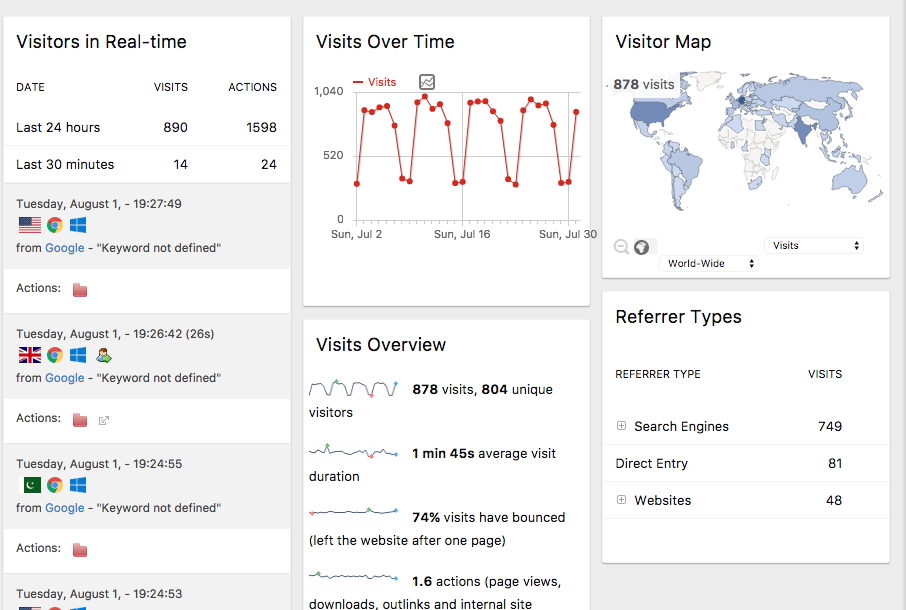
\includegraphics[width = 0.5\textwidth]{screenshots/piwik_home}} &
		\subcaptionbox{
		Piwik: engagement user information \vspace{2 mm}
		\label{fig:piwik_home}}{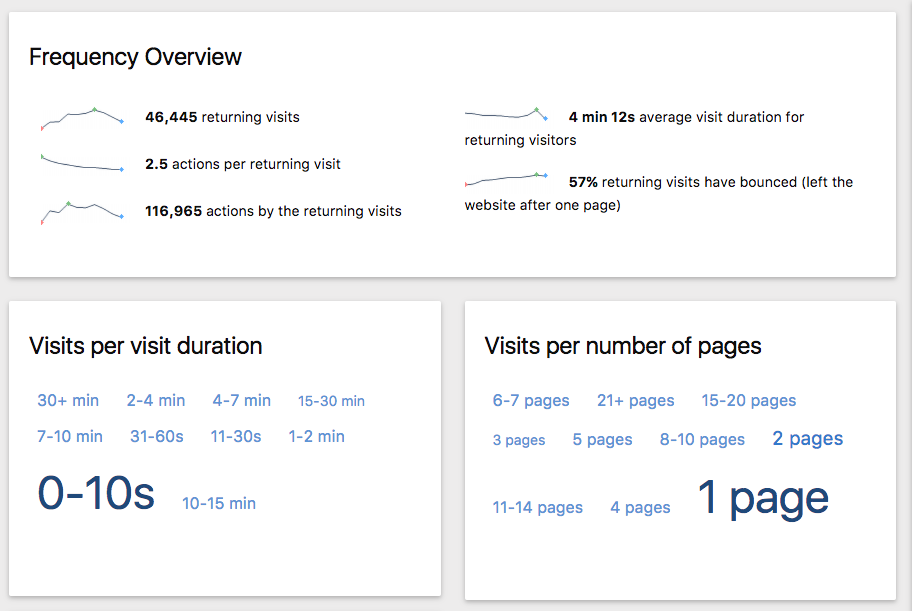
\includegraphics[width = 0.5\textwidth]{screenshots/piwik_engagement}} \\
		\subcaptionbox{
		OWA: home dashboard \vspace{2 mm}
		\label{fig:piwik_home}}{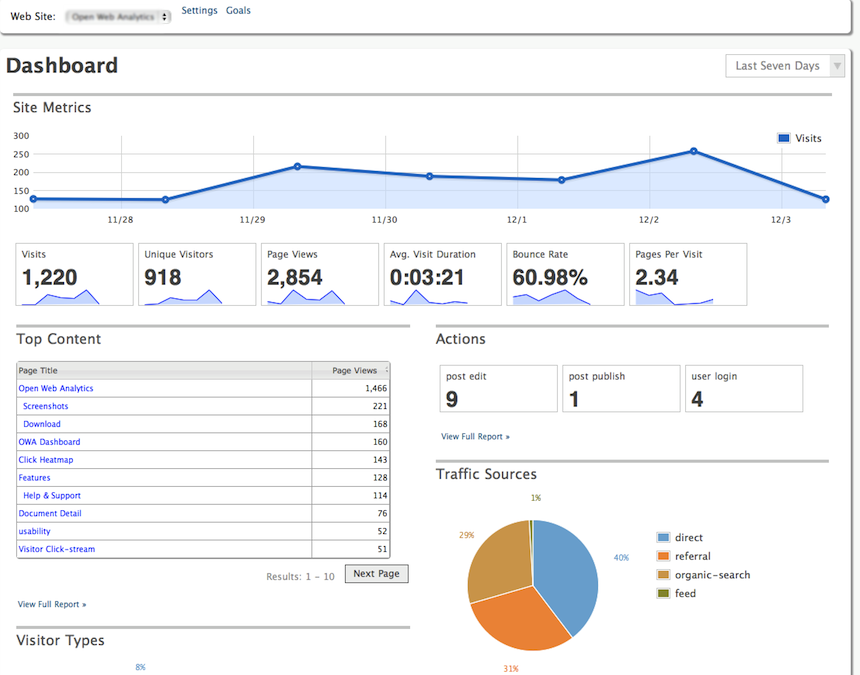
\includegraphics[width = 0.5\textwidth]{screenshots/owa_dashboard}} &
		\subcaptionbox{
		OWA: click heatmap \vspace{2 mm}
		\label{fig:piwik_home}}{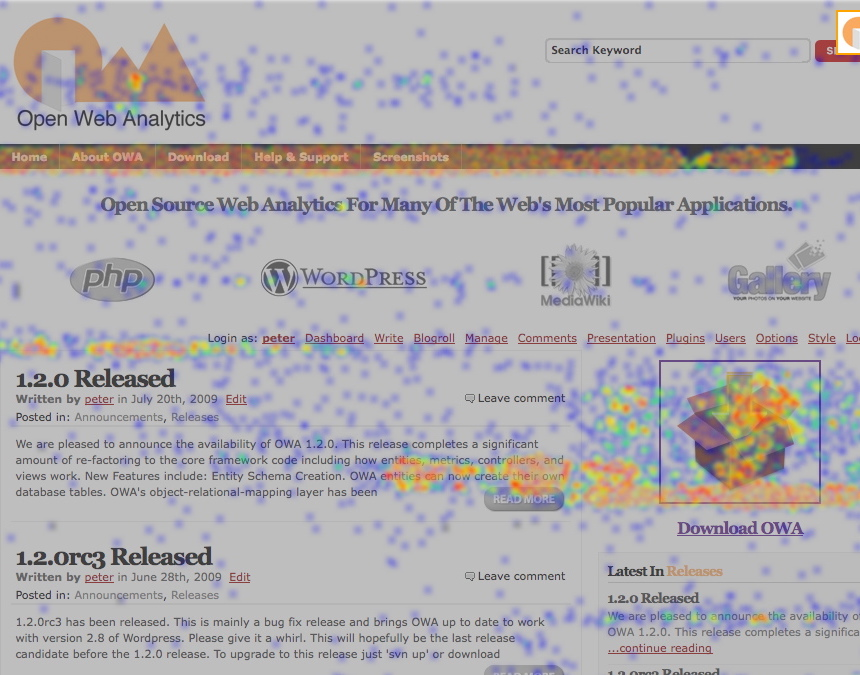
\includegraphics[width = 0.5\textwidth]{screenshots/owa_heatmap}} \\
	\end{tabular}
	\caption{
		Dashboards and reports of some analytics platforms
		\label{fig:screenshots}
	}
\end{figure}

% TODO: previous monitoring tools. Focus in low level data such as network packages and streams

\section{Motivation}
\label{sec:motivation}
Getting insights from the data is a very important skill for any business analyst, marketer or any decision maker. However, it is almost impossible to get knowledge from \textit{raw data}, so it must be presented in a way that is easy to understand and analyze. Luckily, nowadays there are many options to visualize data; as we mentioned in Section~\ref{sec:background} some of those platforms provide tools for doing such tasks, and by the use of geographic maps, pivot tables, heatmaps and other visualization techniques, spotting valuable information becomes easier. Nevertheless, the trend of creating new ways to display web analytics has not been changing much in the past few years, objective reports, conversions and site performance usually are still displayed as tables or big score counters. Figures XYZ shows an example of those reports.

This research propose new ways to display website traffic by using an interactive tool that provides several ways to arrange visits, conversions, user behavior, click stream, pages and filtering options which combined with, for example, Machine Learning pattern recognition, could spot clusters for new market niches or common visitor segments.

% HINT: previous info could be used for intro/abstract

\section{Methodology}
\label{sec:methodology}
The main objective of this research was to use other ways to display visitors and their information in a more graphically way, rather than using tables and counters. To this end, we experimented some techniques such as \textit{treemaps}, \textit{heatmaps} and \textit{network graphs}. Due to the nature of the Internet being a network of connected computers, we decided to base us in network graphs. Following this decision, we needed a support library to compute and display network graphs in many layouts and one of the most popular available is Cytoscape, which was developed by the University of Toronto \cite{}. There are another alternatives like D3.js \cite{} or even Sigma.js \cite{} but Cytoscape has a more friendly programming interface and also it includes a powerful feature to make \textit{queries}. Cytoscape provides a bunch of graph theory algorithms such as \textit{Dijkstra shortest path} \cite{}, \textit{aStar search \cite{}, MST algorithms \cite{}, BFS/DFS traversing and even PageRank \cite{} and centrality algorithms \cite{}.}

Taking advantage of this library we build a web application written in ECMAScript 6 and as a front-end framework, we chose Facebook's React \cite{}.

\subsection{Data collection}
In order to collect the information from visitors, we mounted a website and used one of the tools previously mentioned in Section~\ref{sec:background}: Piwik. This was because it allowed us to gather a lot more of raw information and so we could manipulate it to our needs, things that we could not make if we would use for example Google Analytics. Also there was the problem of getting traffic; we generated \textit{fake traffic} by using HTTP botnets \cite{} but there were also some days of human traffic to the website.


\section{Results}
\label{sec:results}
The motivation of this research was not to build something that magically at first sight you could spot the information you are searching for. Instead, we think that each business, each scenario, each website provides information in a unique way and because of that each \textit{analysis process} is different. Following this philosophy, the analyst just needs the tools and he/she will make use the most of it to find what is important. The work proposed in this research is intended for that; the tool is there, now use it and find useful information.
In order to accomplish this task, of course, the tool must provide useful features, and the one proposed in this work has some interesting ones. Lets take a loot to some of them.

% TODO: Figure

\subsection{Main interface}
The user interface is split in two main areas: the network graph on the left side, and the details pane on the right side.
All the information is displayed given the date range selected in the top bar; there is also the possibility to change that time period.

\subsection{Data representation}
\textbf{Visits}. Each visit is represented an \textit{orange} circle.

\textbf{Pages}. Represented as \textit{blue} circles.

\textbf{Objectives}. For pages marked as \textit{goals or objectives} there is a different color to highlight them, so the \textit{green} circles are used.

Figure XYZ shows the circle's style and how they are connected between them. Each \textit{visit node} is connected to one or more \textit{page/objective nodes} an thus, the connection represents a single visit.
% TODO: display figure

The tool aims to provide easy ways to represent and style the nodes. For example you would be able to chose the size of the circle depending on a metric. For example, making bigger page nodes depending on the number of page views it receives.
The same principle could be applied to visits by the use of metrics like \textit{visit duration, visit count, number of actions made, etc.} And for the case of objective pages a good indicator would be the \textit{bounce rate}.


\subsection{Click Path}
This feature provides a detailed view of how a specific user is browsing inside the website. It is displayed again as a graph but using a DAG (Directed Acyclic Graph) \cite{} layout. Such graph starts with an orange node (the visit) and it should end in a page node.
Intuitively in that path there should be at least one or more green circles, representing that the user reached a goal and so making a conversion for the business.

This is a powerful view of how users are navigating in the website, contrasted with tables or lists which are used by some tools (Figure XYZ), by using a graph we can spot more easily the complexity of the visit.
This could be useful for example to detect behavior. As it was mentioned in Section~\ref{sec:methodology}, there was traffic generated by bots and humans in this research and the \textit{ClickPath} feature can spot clearly the differences between the navigation complexity. As you can see in Figure XYZ, human traffic shows a more complex navigation than bots.

% TODO: figure: comparison of table report vs graphically
% TODO: figure: clickpath bots vs humans

\subsection{Segmentation}
One of the first tasks when you start analyzing an audience is to create segments, which is no more than performing a filter process given a series of conditions;
e.g. young people (\texttt{a < age < b}), men living in New York City (\texttt{gender = 'male' \&\& location = 'NYC'}), people coming from social networks (\texttt{referrer IN ['Facebook', 'Twitter', 'Snapchat']}), etc. So it is very important to have an easy way to perform such filters and because of that, there is a \textit{querying} console incorporated in the tool. This work is presenting only the user interface to access the already built-in Cytoscape's querying system.
% TODO: point part of the screen where it is
The following are examples of queries you can make using the tool, supporting the base logic operators: \textit{AND, OR, NOT, relational operators ($=, >, <, \leq, \geq$), string matching} and others. The full capabilities are provided by Cytoscape and the full specification can be found in the documentation \cite{}. The aim of this section is to provide examples of how to use such query system to our advantage to create segments.
% http://js.cytoscape.org/#selectors/data

\subsubsection{Query format}
Depending on how your data is structured and the available attributes, you would be able to perform queries matching such attributes. We are using data coming from Piwik so we are able to query visits and pages based on their database structure \cite{}.
The format follows the next grammar:
\[
group[ attr \; OP \; value ]
\]

Where:

$ group \in node, edge, className $

$className$ represent a custom class assigned to a particular data. In our case we have three classes: \texttt{visit, page, objective}. So instead of using \textit{node or edge}, we use such classes which is less abstract.

$attr$ means the attribute that you are using as a filter. Such attributes should correspond to the context represented by the \textit{group}. So for example, for the \textit{visits} group, you could have attributes like \texttt{duration, country, browser, events, etc.}; on other hand, in the case of the \textit{page} group you could have attributes like \texttt{url, visits, pageviews, bounceRate, exitRate, avgTimeSpent, etc}.

$OP$ represents any binary operator. Depending of the \textit{data type} you would use one of another. The available operators are: \texttt{=, !=, >, <, >=, <=, *=, $\land$=, \$=}. The last three operators are used for string comparison.

$value$ is the value used for matching $attr$ by the selected operator ($OP$). Depending of the \textit{data type} of \textit{attr} you would put strings, numbers or booleans.

\subsubsection{Logical operators}
To implement the logical operators \textit{AND, OR} you have to follow the next format:

\textbf{AND}:
\[
group[attr_1 \; OP_1 \; value_1]group_2[attr_2 \; OP_2 \; value_2] \; \ldots \; [attr_n \; OP_n \; value_n]
\]
Notice the join of groups after the square brackets.

\textbf{OR}:
\[
group[attr_1 \; OP \; value_1],group_2[ attr_2 \; OP \; value_2]
\]

Notice the use of the \textit{comma ($,$)} for concatenating conditions.

\subsubsection{Examples and use cases}
\label{sec:examples}
Visitors from the United States:
\begin{lstlisting}
.visit[countryCode = "us"]
\end{lstlisting}

Visitors using Google Chrome \textit{and} with a visit duration greater than 10 seconds \textit{and} that are from South America.
\begin{lstlisting}
.visit[browserCode = 'CH'][visitDuration > 10][continentCode = 'ams']
\end{lstlisting}

An interesting use case for the previous querying system enables us to use it with \textbf{Machine Learning} algorithms, specifically with decision trees based techniques that create patterns splitting the data by attribute values. The figure XYZ shows a J48 decision tree \cite{} trained with traffic data, spotting clusters of visitors that match certain properties.

\subsection{Insight through layouts}

Positioning the nodes in a clever way could result into instant insights from your site and how it is performing. By default Cytoscape provides several layouts to arrange the node, some of them would position the nodes depending on the graph's attributes like the node's \textit{degree}, connected components or betweenness centrality. Default layouts included in the library are: \textit{grid, random, preset, circle, concentric, breadth first, cose.}
It also has extensions to use third-party layouts like Cose and Cose-Bilkent \cite{} (often used in micro-biology), Cola \cite{} or force layouts \cite{} which simulate gravity attraction. It is the decision of the analyzer to use the layout that seems to fit better to the situation, choosing the right one could improve the way to discover new patterns.

However, we propose the use of the \textit{concentric layout} to give an indicator of one of the most used metrics in web analytics: \textit{bounce rate}. The motivation is to \textit{keep in the closest radius your objective pages}, meaning a good performance the more of they are in the first concentric circle. This enables the analyst to start asking the right questions.
The following cases are possible situations of \textit{performance indicators} like \textit{bounce rate}, we believe that using the \textit{concentric layout} would be a good way to spot such performance and also to discover new opportunities in the website pages. The metric used for the reports is \textit{bounce rate}.

\textbf{Case 1: green nodes in the first level.}

This is a good indicator representing that your objectives are \textit{healthy}, meaning that your are accomplishing all of your objectives, because all of them are in the first concentric level. Of course this would be the \textit{ideal case} for any business.

\textbf{Case 2: green nodes spread in many levels.}

Another way to spot how your objectives are performing. The intuition here is that if the green nodes are far from the first level, then it means that you should improve them. It also serves as an indicator to \textit{track performance}: for example, you can define \textit{how many levels your objective has jumped since previous auditing.}

\textbf{Case 3: blue and green nodes mixed in the closest levels.}

Although at first sight you can think that it is not a good indicator to have \textit{blue circles} inside your first level, \textit{you can take advantage of it.}
Because this is telling you that you have pages that can lead to \textit{potential conversions}, therefore, you should try to use them to engage your users. Possible use cases for those pages are inserting in them call-to-action elements, displaying ads, making offers or treat them as landing pages. Again, you can use this knowledge to engage the users and lead them to a conversion.

% TODO: Figure with the three cases


\section{Conclusions}
Helps to see graphically metrics of user behavior

Future work
Setting up as a recommendation system to spot new segments
Auto complete system
Improve layout
Aggregate elements
Use node compression

%% References
%%
%% Following citation commands can be used in the body text:
%% Usage of \cite is as follows:
%%   \cite{key}         ==>>  [#]
%%   \cite[chap. 2]{key} ==>> [#, chap. 2]
%%

%% References with bibTeX database:

\bibliographystyle{elsarticle-num}
% \bibliographystyle{elsarticle-harv}
% \bibliographystyle{elsarticle-num-names}
% \bibliographystyle{model1a-num-names}
% \bibliographystyle{model1b-num-names}
% \bibliographystyle{model1c-num-names}
% \bibliographystyle{model1-num-names}
% \bibliographystyle{model2-names}
% \bibliographystyle{model3a-num-names}
% \bibliographystyle{model3-num-names}
% \bibliographystyle{model4-names}
% \bibliographystyle{model5-names}
% \bibliographystyle{model6-num-names}

\bibliography{references}


\end{document}

%%
%% End of file `elsarticle-template-num.tex'.
